%!TEX root = ../thesis.tex

\section{実験1:2DLiDARの反射強度の実験}

  実験1では,2DLiDARの反射強度を利用した実験を行う.ここでは,以下に示す3つの事項に関して調査する.なお,以下の実験では,2DLiDARの検出範囲を0 \,[rad]で更に制限している.
  % 4の実験では,提案手法通り最大2.094 \,[rad](120 \,[deg])の範囲で検出する.

  \begin{enumerate}
    \item 壁の反射強度を計測する実験
    \item 再帰反射テープの反射強度を計測する実験
    \item 学習フェーズで使用する周辺環境の反射強度を計測する実験
    % \item ルールベース制御器を用いた人追従の実験
  \end{enumerate}

\subsection{実験目的}

本研究では,2DLiDARの反射強度を利用したルールベース制御器を用いた人追従行動を,カメラ画像で模倣学習することを課題としている.ルールベース制御器は,最大反射強度の方にロボットが追従する手法となっているため,実験で使用する再帰反射テープよりも高い反射強度を取得してしまうと人追従行動を継続できない恐れがある.そのため,実験場所として指定した,千葉工業大学津田沼キャンパス2号館3階の廊下において,再帰反射テープよりも反射強度の高いものが存在しないかを,実験により調査する.

\newpage

\subsection{壁の反射強度}

  実験場所である,千葉工業大学津田沼キャンパス2号館3階の廊下の壁の反射強度を計測した.実験の様子を\figref{Fig:RobotGuidance_exp1_wall}に示す.2DLiDARを壁に向けて正面に配置し,距離によって反射強度の値が変化するのを防ぐため,壁から約500 \,[mm]離れたところに固定した.
  
  計測した結果を\figref{Fig:Normal distribution of reflection intensity of wall}に示す.収集したデータは1万個で,平均値は約3600であり,平均値付近にデータが集中していることがわかった.

  \begin{figure}[h]
    \centering
    \begin{minipage}[c]{65mm} 
        \centering
        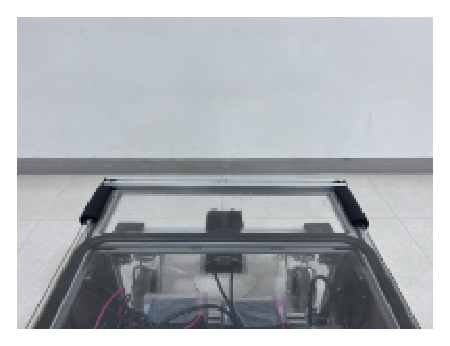
\includegraphics[height=40mm]{images/eps/RobotGuidance_exp1_wall_from_back}
        \subcaption{View from behind}
    \end{minipage}
    \begin{minipage}[c]{65mm} 
        \centering
        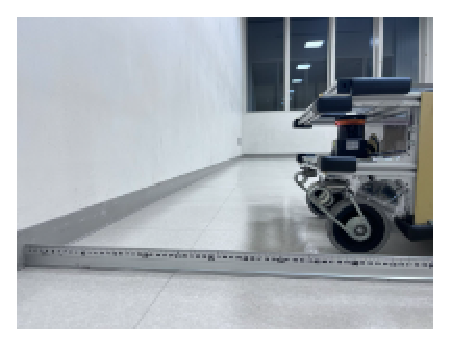
\includegraphics[height=40mm]{images/eps/RobotGuidance_exp1_wall_from_side}
        \subcaption{View from the side}
    \end{minipage}
    \caption{Measure the reflection intensity of the wall}
    \label{Fig:RobotGuidance_exp1_wall}
  \end{figure}

  \begin{figure}[h]
    \centering
    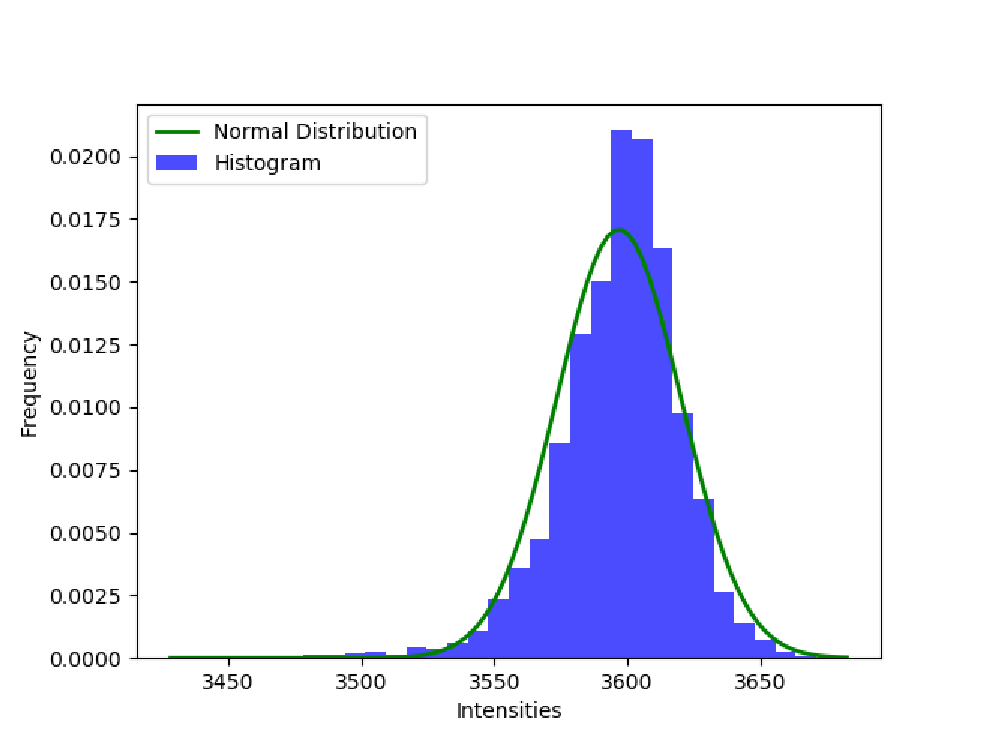
\includegraphics[keepaspectratio, scale=0.50] {images/eps/RobotGuidance_plot_reflection_intensities_of_wall}
    \captionsetup{justification=raggedright} % キャプションを左寄せに
    \caption{Normal distribution of reflection intensity of wall}
    \label{Fig:Normal distribution of reflection intensity of wall}
  \end{figure}

\newpage

\subsection{再帰反射テープの反射強度}

  再帰反射テープの反射強度を計測した.実験の様子を\figref{Fig:RobotGuidance_exp2_tape}に示す.2DLiDARを再帰反射テープに向けて正面に配置し,距離によって反射強度の値が変化するのを防ぐため,再帰反射テープから約500 \,[mm]離れたところに固定した.
    
  計測した結果を\figref{Fig:Normal distribution of reflection intensity of retroreflective tape}に示す.収集したデータは1万個で,平均値は約15300であり,平均値付近にデータが集中していることがわかった.

  \begin{figure}[h]
    \centering
    \begin{minipage}[c]{65mm} 
        \centering
        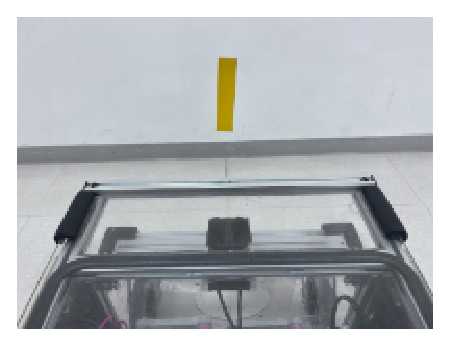
\includegraphics[height=40mm]{images/eps/RobotGuidance_exp2_tape_from_back}
        \subcaption{View from behind}
    \end{minipage}
    \begin{minipage}[c]{65mm} 
        \centering
        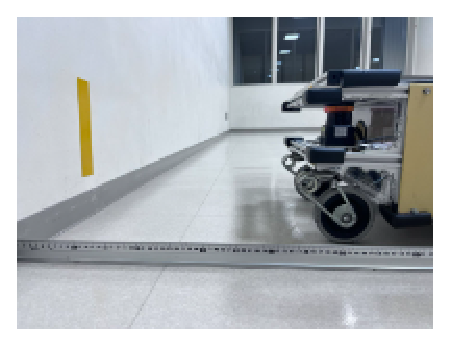
\includegraphics[height=40mm]{images/eps/RobotGuidance_exp2_tape_from_side}
        \subcaption{View from the side}
    \end{minipage}
    \caption{Measure the reflection intensity of retroreflective tape}
    \label{Fig:RobotGuidance_exp2_tape}
  \end{figure}

  \begin{figure}[h]
    \centering
    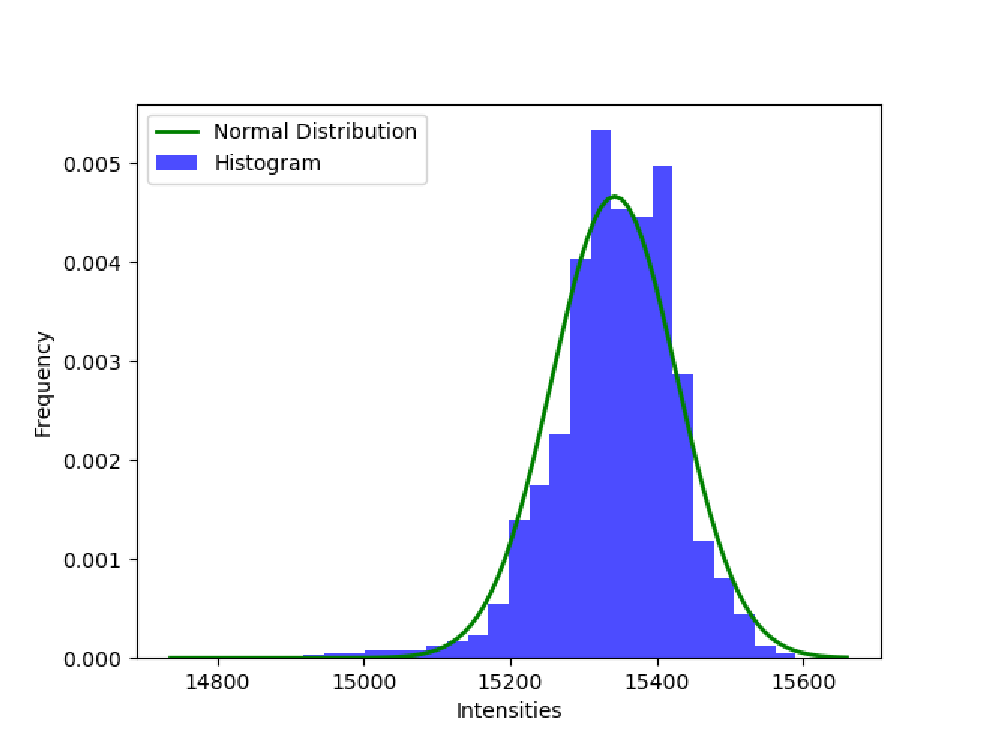
\includegraphics[keepaspectratio, scale=0.50] {images/eps/RobotGuidance_plot_reflection_intensities_of_tape}
    \captionsetup{justification=raggedright} % キャプションを左寄せに
    \caption{Normal distribution of reflection intensity of retroreflective tape}
    \label{Fig:Normal distribution of reflection intensity of retroreflective tape}
  \end{figure}

\newpage

\subsection{学習する場所付近の反射強度}

  学習フェーズで使用する場所を\figref{Fig:RobotGuidance_exp3_foyer}に示す.ここは,千葉工業大学津田沼キャンパス2号館3階のホワイエと呼ばれるスペースであり,中にはガラスや自動販売機が存在する.それぞれに対して反射強度を計測するのは大変なので,ホワイエをランダムに歩き回ることでデータを収集する.

  計測した結果を\figref{Fig:Histogram of reflection intensity of foyer}に示す.収集したデータは1万個で,ホワイエには5000を超える反射強度の値は存在しないことがわかった.つまり,再帰反射テープが最大反射強度であり,ルールベース制御器が正常に機能すると,人追従行動生成が可能であることを確認した.

  \begin{figure}[h]
    \centering
    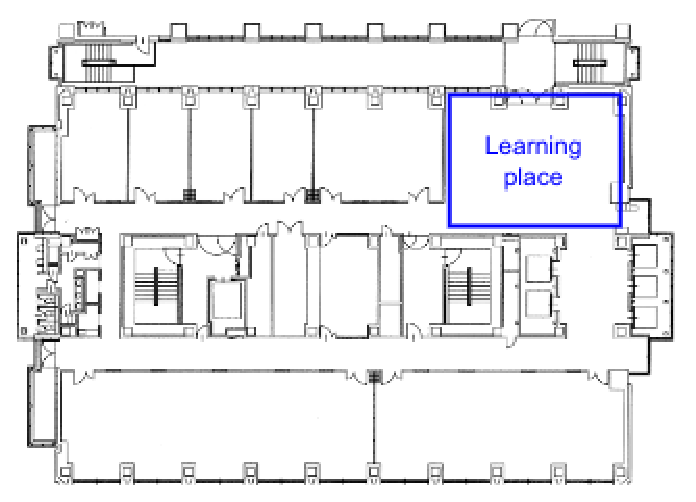
\includegraphics[keepaspectratio, scale=0.50] {images/eps/RobotGuidance_exp3_foyer}
    \captionsetup{justification=raggedright} % キャプションを左寄せに
    \caption{Measure the reflection intensity of foyer}
    \label{Fig:RobotGuidance_exp3_foyer}
  \end{figure}

  \begin{figure}[h]
    \centering
    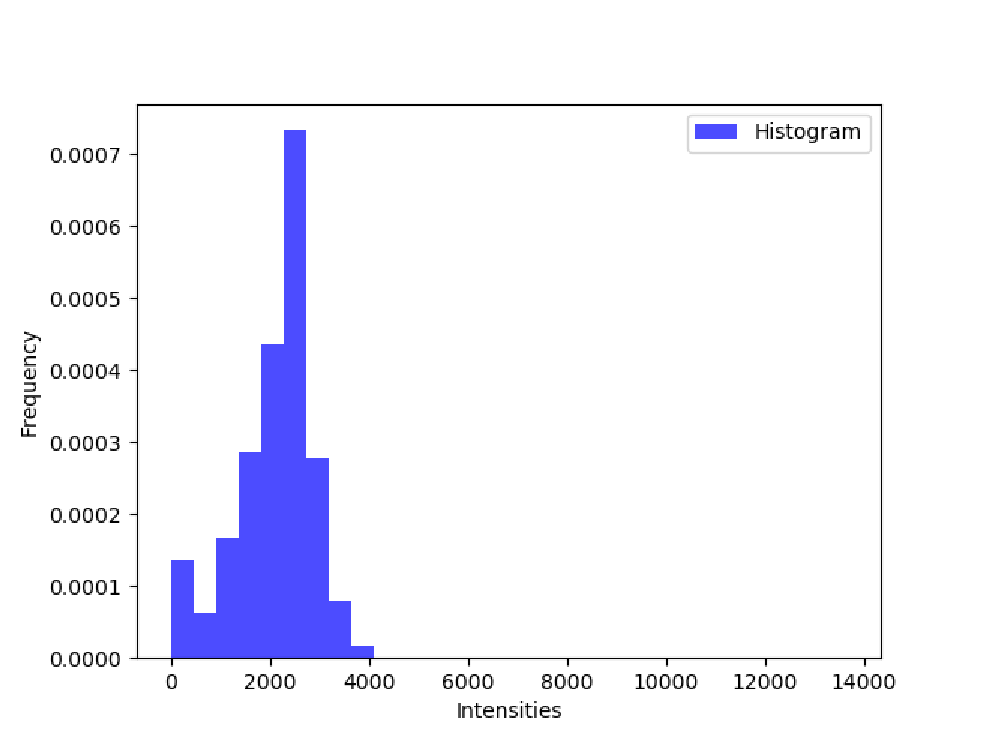
\includegraphics[keepaspectratio, scale=0.50] {images/eps/RobotGuidance_plot_reflection_intensities_of_foyer}
    \captionsetup{justification=raggedright} % キャプションを左寄せに
    \caption{Histogram of reflection intensity of foyer}
    \label{Fig:Histogram of reflection intensity of foyer}
  \end{figure}

\newpage

% \subsection{反射強度を利用した人追従の実験}

%   2DLiDARの反射強度を利用した人追従の実験を行う.この実験により,ルールベース制御器がホワイエにて有効であるか明らかにする.実験の様子を\figref{Fig:Parson following behavior using rule-based controller}に示す.10分間,ホワイエをランダムに歩き回り,その間のルールベース制御器によるロボットの挙動を観察した.その結果,ロボットはルールベース制御器に従い,10分間にわたり人を追従し続け,その有効性を確認した.

%   \begin{figure}[h]
%     \centering
%     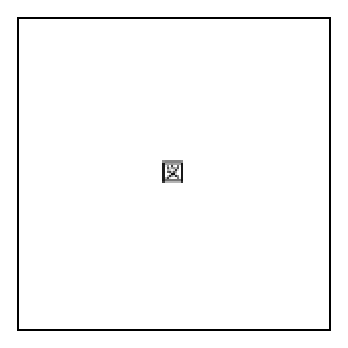
\includegraphics[keepaspectratio, scale=0.80] {images/eps/figure}
%     \captionsetup{justification=raggedright} % キャプションを左寄せに
%     \caption{Parson following behavior using rule-based controller}
%     \label{Fig:Parson following behavior using rule-based controller}
%   \end{figure}

% \newpage
